% Provenance (never printed): see sources/outline_sources.md and sources/book1/BRIEFS.md (g1/02).
\chapter{Instructions in Order}\label{ch:g1:instructions-in-order}

Tom's little brother Leo is hungry. Tom has to go out, so he writes the steps
for making a jam sandwich on a piece of paper: ``Spread jam on a slice of
bread. Open the jar. Take two slices of bread. Put one slice on the other.''
Leo follows the steps exactly as they are written. He tries to spread jam
with the jar still closed. Then he opens the jar, and only then does he take
the bread. When Tom comes back, the kitchen is a mess.

Every step on Tom's paper was right. What went wrong was their order. A
\omterm{def:g1:what-is-a-computer:computer}{computer} is like Leo: it follows the steps it is given, exactly, in the order
they are given.

\begin{recall}
A \omterm{def:g1:what-is-a-computer:computer}{computer} is a machine that follows \omterm{def:g1:instructions-in-order:instruction}{instructions}
(\cref{ch:g1:what-is-a-computer}). People write the \omterm{def:g1:instructions-in-order:instruction}{instructions}; the
\omterm{def:g1:what-is-a-computer:computer}{computer} carries them out, very fast, and nothing else.
\end{recall}

\section{A task as a list of steps}

Many things we do every day are made of steps: making a sandwich, getting
dressed, brushing our teeth, planting a seed. To tell somebody how to do such
a task, we can write the steps one under the other.

\begin{definition}[Instruction]\label{def:g1:instructions-in-order:instruction}
An \emph{instruction}\index{instruction} is one step that tells exactly what
to do: ``take two slices of bread'', ``turn left'', ``stop''.
\end{definition}

A good \omterm{def:g1:instructions-in-order:instruction}{instruction} is short and clear. ``Make the sandwich nicely'' is not a
good \omterm{def:g1:instructions-in-order:instruction}{instruction}: Leo cannot know what ``nicely'' means. ``Cut the sandwich
in two'' is clear.

\begin{example}[Brushing your teeth]\label{ex:g1:instructions-in-order:teeth}
1.~Wet the toothbrush. 2.~Put toothpaste on the toothbrush. 3.~Brush your
teeth for two minutes. 4.~Rinse your mouth. 5.~Rinse the toothbrush. Each line
is one \omterm{def:g1:instructions-in-order:instruction}{instruction}.
\end{example}

\section{The order matters}

\begin{definition}[Sequence of instructions]\label{def:g1:instructions-in-order:sequence}
A \emph{sequence of instructions}\index{sequence of instructions} is a list of
\omterm{def:g1:instructions-in-order:instruction}{instructions} to follow one after the other, from the first to the last, in
the order in which they are written.
\end{definition}

If two steps are swapped, the result can be wrong. You must put on your socks
before your shoes. Tom's sandwich went wrong because ``open the jar'' came
after ``spread jam''.

\begin{omfigure}
\begin{tikzpicture}[x=1cm, y=1cm, font=\small,
    card/.style={draw=black!60, rounded corners=3pt, fill=ocPaleBlue, text width=2.25cm,
      minimum height=1.5cm, align=center, inner sep=3pt},
    bad/.style={card, fill=ocRed!15},
    num/.style={circle, draw=black!60, fill=white, inner sep=1pt, font=\scriptsize\bfseries}]
  \node[anchor=west, font=\bfseries] at (-1.3,2.15) {Right order};
  \foreach \t [count=\k] in {Take two slices of bread, Open the jar of jam,
      Spread jam on one slice, Put the other slice on top, Cut the sandwich in two} {
    \node[card] (c\k) at ({2.6*(\k-1)},1) {\t};
    \node[num] at (c\k.north west) {\k};
  }
  \node[anchor=west, font=\bfseries] at (-1.3,-0.65) {Steps 2 and 3 swapped};
  \foreach \t/\s [count=\k] in {Take two slices of bread/card, Spread jam on one slice/bad,
      Open the jar of jam/bad, Put the other slice on top/card, Cut the sandwich in two/card} {
    \node[\s] (d\k) at ({2.6*(\k-1)},-1.8) {\t};
    \node[num] at (d\k.north west) {\k};
  }
  \node[font=\footnotesize, text=ocRed!80!black, align=center] at (2.6,-3.0) {the jar is still closed!};
\end{tikzpicture}

{\small The same five \omterm{def:g1:instructions-in-order:instruction}{instructions} in two orders. With steps 2 and 3 swapped,
the jam cannot be spread: the jar is still closed.}
\label{fig:g1:instructions-in-order:sandwich}
\end{omfigure}

Sometimes two steps can be swapped without any harm. You can put on your left
glove first or your right glove first: both orders give two warm hands. Before
you change the order of two steps, ask yourself: does the second step need the
first one to be done?

\section{Guiding a robot on a grid}

In the classroom, Mia and Sami play with a small floor robot on a mat made of
squares. The robot understands only three \omterm{def:g1:instructions-in-order:instruction}{instructions}:
\begin{itemize}
\item \textbf{forward} ($\uparrow$): move one square forward, in the direction
it faces;
\item \textbf{left} ($\circlearrowleft$): turn a quarter turn to the left, on
the spot, without moving to another square;
\item \textbf{right} ($\circlearrowright$): turn a quarter turn to the right,
on the spot.
\end{itemize}

\begin{omfigure}
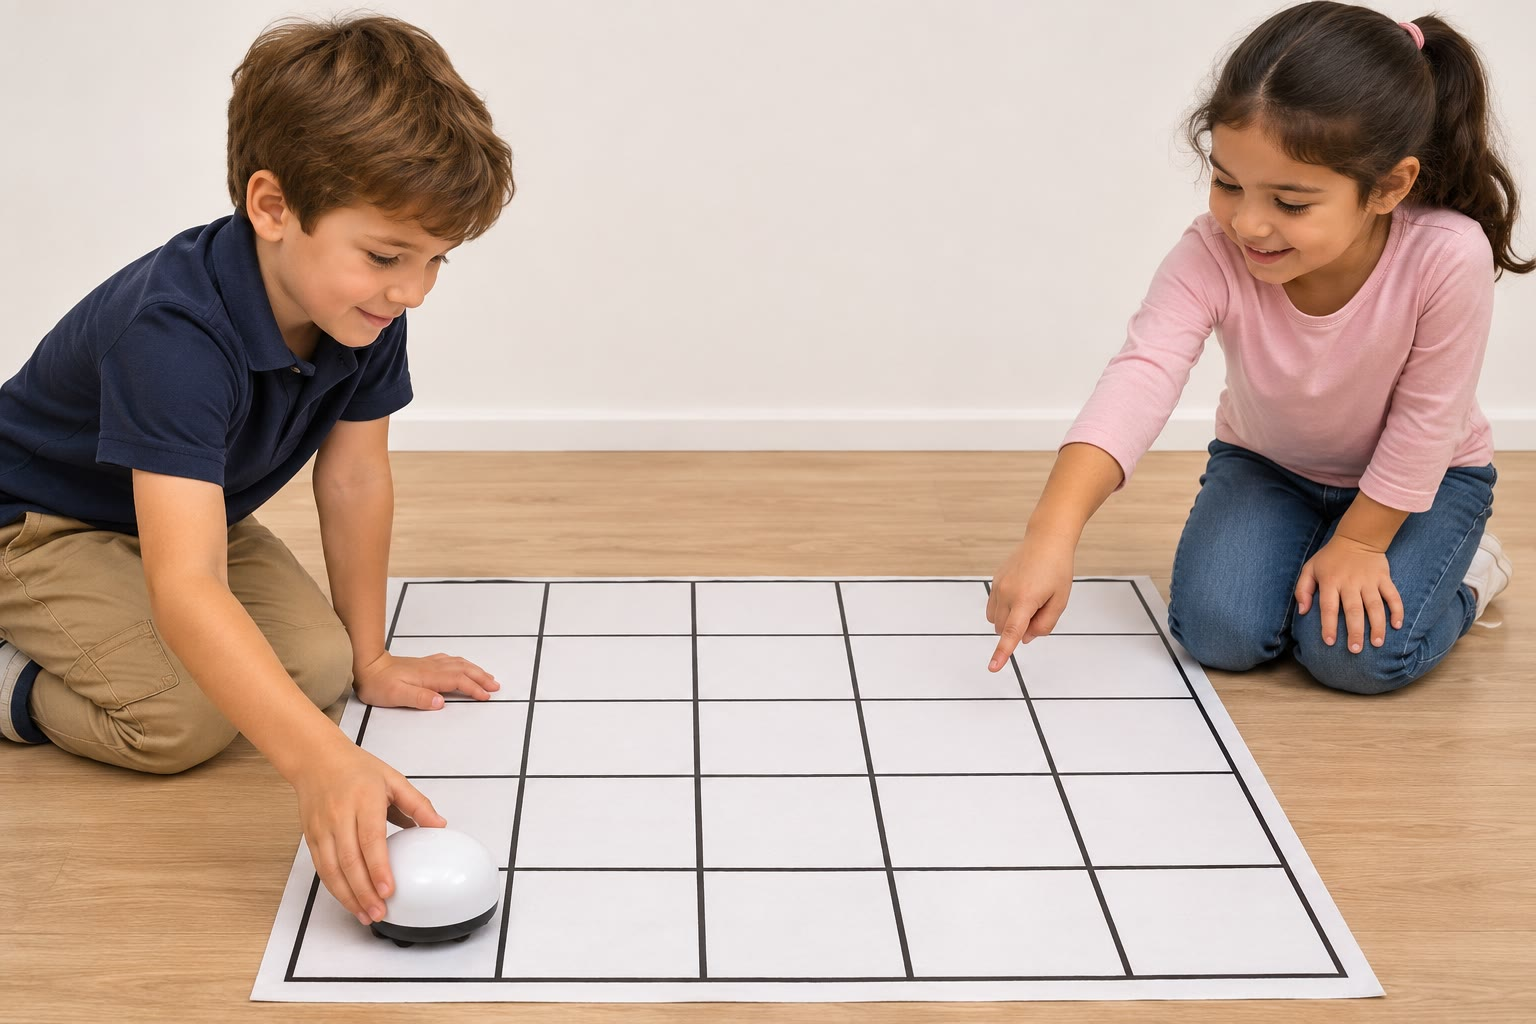
\includegraphics[width=0.6\linewidth]{images/book1/ai/g1-instructions-in-order-floor-robot.jpg}

{\small A floor robot on a mat of squares. The children give it a \omterm{def:g1:instructions-in-order:sequence}{sequence of
instructions}, then press start.}
\end{omfigure}

\begin{omfigure}
\begin{tikzpicture}[x=1cm, y=1cm, font=\small]
  \foreach \cx/\name/\sym/\d in {0/forward/{$\uparrow$}/0, 4.5/left/{$\circlearrowleft$}/1, 9/right/{$\circlearrowright$}/2} {
    \begin{scope}[shift={(\cx,0)}]
      \node[font=\bfseries] at (1.5,2.9) {\name\quad\sym};
      % before
      \draw[black!40] (0,0) grid (1,2);
      \draw[black!40] (2,0) grid (3,2);
      \node[font=\scriptsize] at (0.5,-0.3) {before};
      \node[font=\scriptsize] at (2.5,-0.3) {after};
      \draw[-{Stealth[length=2mm]}, black!50] (1.15,1) -- (1.85,1);
      \fill[ocBlue!60] (0.5,0.5) circle (0.3); \fill[white] (0.5,0.72) circle (0.07);
      \ifnum\d=0
        \fill[ocBlue!60] (2.5,1.5) circle (0.3); \fill[white] (2.5,1.72) circle (0.07);
      \fi
      \ifnum\d=1
        \fill[ocBlue!60] (2.5,0.5) circle (0.3); \fill[white] (2.28,0.5) circle (0.07);
      \fi
      \ifnum\d=2
        \fill[ocBlue!60] (2.5,0.5) circle (0.3); \fill[white] (2.72,0.5) circle (0.07);
      \fi
    \end{scope}
  }
\end{tikzpicture}

{\small The three \omterm{def:g1:instructions-in-order:instruction}{instructions} of the robot. The white dot shows where the
robot faces. ``Forward'' moves it one square; ``left'' and ``right'' only
turn it on its square.}
\label{fig:g1:instructions-in-order:three}
\end{omfigure}

We write a sequence for the robot as a row of \omterm{def:g1:instructions-in-order:instruction}{instructions}, read from left to
right. The robot starts on the square marked S, facing to the right.

\begin{example}[Reaching the star]\label{ex:g1:instructions-in-order:star}
Mia writes the sequence
\[
\uparrow\ \uparrow\ \circlearrowleft\ \uparrow\ \uparrow\ \circlearrowright\ \uparrow
\]
(forward, forward, left, forward, forward, right, forward). The robot goes two
squares to the right, turns to face up, goes up two squares, turns to face
right again, and goes one more square. It stops on the star. The drawing below
shows its path.
\end{example}

\begin{omfigure}
\begin{tikzpicture}[x=0.9cm, y=0.9cm, font=\small]
  \draw[black!35] (0,0) grid (6,5);
  \node[font=\bfseries] at (0.5,0.5) {S};
  \node[star, star points=5, star point ratio=2.2, fill=ocYellow, draw=black!60, inner sep=1.6pt] at (3.5,2.5) {};
  \draw[ocBlue, line width=1.6pt, -{Stealth[length=3mm]}] (0.5,0.5) -- (2.5,0.5) -- (2.5,2.5) -- (3.2,2.5);
  \foreach \x/\y/\t in {1.5/0.5/1, 2.5/0.5/2, 2.5/1.5/4, 2.5/2.5/5, 3.5/2.5/7}
    \node[font=\scriptsize, text=ocBlue!80!black, anchor=north west, inner sep=1pt] at (\x-0.45,\y+0.45) {\t};
  \node[anchor=west, align=left, font=\small] at (6.4,2.5)
    {$\uparrow\ \uparrow\ \circlearrowleft\ \uparrow\ \uparrow\ \circlearrowright\ \uparrow$\\[2pt]
     {\footnotesize the small numbers tell after which}\\{\footnotesize instruction the robot is on each square}};
\end{tikzpicture}

{\small The path of the robot for Mia's sequence. It starts on S, facing to
the right, and stops on the star.}
\label{fig:g1:instructions-in-order:grid}
\end{omfigure}

\begin{remark}[Turning does not move]\label{rem:g1:instructions-in-order:turn}
After ``left'' or ``right'' the robot is still on the same square: only the
direction it faces has changed. That is why no square of the drawing carries
the numbers 3 and 6: \omterm{def:g1:instructions-in-order:instruction}{instructions} 3 and 6 are turns.
\end{remark}

\section{Finding the wrong step}

Sami wants the robot to reach the flag. He writes
\[
\uparrow\ \uparrow\ \uparrow\ \circlearrowleft\ \uparrow\ \uparrow\ \uparrow\ \uparrow
\]
but the robot stops far from the flag. Which \omterm{def:g1:instructions-in-order:instruction}{instruction} is wrong?

\begin{method}[Finding a wrong instruction]\label{met:g1:instructions-in-order:wrong-step}
Put your finger on the start square, facing the right way. Read the sequence
one \omterm{def:g1:instructions-in-order:instruction}{instruction} at a time and move your finger for each one, as the robot
would. After each \omterm{def:g1:instructions-in-order:instruction}{instruction}, check: is the finger still on a good path to
the goal? The first \omterm{def:g1:instructions-in-order:instruction}{instruction} after which the answer is ``no'' is the wrong
one. Change only that \omterm{def:g1:instructions-in-order:instruction}{instruction}, then follow the whole sequence again from
the start.
\end{method}

\begin{omfigure}
\begin{tikzpicture}[x=0.8cm, y=0.8cm, font=\small]
  \foreach \ox/\title in {0/Sami's sequence, 8/the fixed sequence} {
    \begin{scope}[shift={(\ox,0)}]
      \draw[black!35] (0,0) grid (6,5);
      \node[font=\bfseries] at (0.5,0.5) {S};
      \draw[black!70, fill=ocRed!60] (4.5,3.2) -- (4.5,3.85) -- (4.85,3.65) -- (4.5,3.45);
      \draw[black!70, line width=0.8pt] (4.5,3.15) -- (4.5,3.85);
      \node[font=\bfseries] at (3,5.45) {\title};
    \end{scope}
  }
  \draw[ocRed!80!black, line width=1.6pt, -{Stealth[length=3mm]}] (0.5,0.5) -- (3.5,0.5) -- (3.5,4.25);
  \node[font=\scriptsize, text=ocRed!80!black, anchor=west, align=left, fill=white, inner sep=1pt] at (3.8,1.6) {turns left\\one square\\too early};
  \draw[omMeth, line width=1.6pt, -{Stealth[length=3mm]}] (8.5,0.5) -- (12.5,0.5) -- (12.5,3.25);
  \node[anchor=north, font=\small] at (3,-0.25) {$\uparrow\ \uparrow\ \uparrow\ \circlearrowleft\ \uparrow\ \uparrow\ \uparrow\ \uparrow$};
  \node[anchor=north, font=\small] at (11,-0.25) {$\uparrow\ \uparrow\ \uparrow\ \uparrow\ \circlearrowleft\ \uparrow\ \uparrow\ \uparrow$};
\end{tikzpicture}

{\small Left: Sami's robot turns left after three squares instead of four, so
it goes up the wrong column. Right: with the turn moved one place later, the
robot reaches the flag.}
\label{fig:g1:instructions-in-order:wrong}
\end{omfigure}

\begin{example}[Fixing Sami's sequence]\label{ex:g1:instructions-in-order:fix}
With a finger: forward, forward, forward --- the finger is three squares to
the right of S. The flag is four squares to the right, so the next \omterm{def:g1:instructions-in-order:instruction}{instruction}
should be ``forward'' again, not ``left''. The fourth \omterm{def:g1:instructions-in-order:instruction}{instruction} is the wrong
one. The fixed sequence is forward four times, left, then forward three times:
the robot goes up the column of the flag and stops on it.
\end{example}

\section{Exercises}

Exercises~3 to~10 use the grid below. The robot always starts on S, facing to
the right. The grey squares are walls: the robot cannot enter them.

\begin{omfigure}
\begin{tikzpicture}[x=0.9cm, y=0.9cm, font=\small]
  \fill[black!30] (0,2) rectangle (2,3);
  \draw[black!35] (0,0) grid (6,5);
  \node[font=\bfseries] at (0.5,0.5) {S};
  \foreach \x/\y/\t in {3/2/A, 5/4/B, 2/3/C, 0/4/D}
    \node[circle, draw=black!60, fill=ocYellow!50, inner sep=1.5pt, font=\small\bfseries] at (\x+0.5,\y+0.5) {\t};
\end{tikzpicture}

{\small The grid of the exercises: start S, the squares A, B, C, D, and two
walls.}
\label{fig:g1:instructions-in-order:exercise-grid}
\end{omfigure}

\begin{exercise}[$\star$]\label{exo:g1:instructions-in-order:1}
Put these five steps of getting dressed in a good order: put on your shoes;
put on your coat; put on your socks; put on your trousers; put on your pants.
\end{exercise}

\begin{exercise}[$\star$]\label{exo:g1:instructions-in-order:2}
In the list of exercise~1, find two steps that can be swapped without any
harm, and two steps that cannot.
\end{exercise}

\begin{exercise}[$\star$]\label{exo:g1:instructions-in-order:3}
The robot follows
$\uparrow\ \uparrow\ \circlearrowleft\ \uparrow\ \uparrow\ \uparrow$.
On which letter does it stop?
\end{exercise}

\begin{exercise}[$\star$]\label{exo:g1:instructions-in-order:4}
Write a sequence that takes the robot from S to B.
\end{exercise}

\begin{exercise}[$\star$]\label{exo:g1:instructions-in-order:5}
Lina wants to reach A. She writes
$\uparrow\ \uparrow\ \uparrow\ \uparrow\ \circlearrowleft\ \uparrow\ \uparrow$,
and the robot stops one square to the right of A. Which \omterm{def:g1:instructions-in-order:instruction}{instruction} is wrong?
Write the fixed sequence.
\end{exercise}

\begin{exercise}[$\star$]\label{exo:g1:instructions-in-order:6}
Which of these sequences draws the path of the drawing of Mia's robot
(the path to the star)?
(a)~$\uparrow\ \uparrow\ \circlearrowright\ \uparrow\ \uparrow\ \circlearrowleft\ \uparrow$;
(b)~$\uparrow\ \uparrow\ \circlearrowleft\ \uparrow\ \uparrow\ \circlearrowright\ \uparrow$;
(c)~$\uparrow\ \circlearrowleft\ \uparrow\ \uparrow\ \circlearrowright\ \uparrow\ \uparrow$.
\end{exercise}

\begin{exercise}[$\star$]\label{exo:g1:instructions-in-order:7}
The sequences $\uparrow\ \uparrow\ \uparrow\ \circlearrowleft\ \uparrow\ \uparrow$
and $\uparrow\ \uparrow\ \circlearrowleft\ \uparrow\ \circlearrowright\ \uparrow\ \circlearrowleft\ \uparrow$
both take the robot to the same square. Which square? How many \omterm{def:g1:instructions-in-order:instruction}{instructions}
does each sequence have?
\end{exercise}

\begin{exercise}[$\star\star$]\label{exo:g1:instructions-in-order:8}
Write the shortest sequence you can find that takes the robot from S to D
without entering a wall. How many \omterm{def:g1:instructions-in-order:instruction}{instructions} does it have?
\end{exercise}

\begin{exercise}[$\star\star$]\label{exo:g1:instructions-in-order:9}
Write a sequence that makes the robot leave S and come back to S.
\end{exercise}

\begin{exercise}[$\star\star$]\label{exo:g1:instructions-in-order:10}
The left \omterm{def:g1:instructions-in-order:instruction}{instruction} of the robot is broken: you may only use
$\uparrow$ and $\circlearrowright$. Write a sequence that takes the robot from
S to A.
\end{exercise}
